\chapter{Raspberry Pi Setting}
\label{chp:rpi}

\section{About Raspberry Pi}
\par The \gls{rpi} is a credit-card-sized single-board computer developed in the UK by the Raspberry Pi Foundation with the intention of promoting the teaching of basic computer science in the schools. \cite{rpi} The \gls{rpi} has a Broadcom BCM2835 system on a chip, which includes an ARM1176JZF-S 700 MHz processor (The firmware includes a number of "Turbo" modes so that the user can attempt overclocking, up to 1 GHz, without affecting the warranty), VideoCore IV GPU, and was originally shipped with 256 megabytes of RAM, later upgrade to 512 MB. It does not include a built-in hard disk or solid-state drive, but uses an \gls{sd} card for booting and long-term storage. The Foundation's goal was to offer two versions.
\subsection{\gls{rpi} Hardware for Project}
\par In this project, one Kingston 8 \gls{gb} \gls{sd} card is used instead of previous Samsung 16 \gls{gb} \gls{sd} card in the master project\cite{TorgeirMR} because the Samsung 16 \gls{gb} \gls{sd} card used in the previous project is quite unstable since its root file system has been broken by the voltage changes of the \gls{usb} hub on the \gls{rpi} during the development of this report project. 
\par In this project, it will use model B as the residential access point because the model B is more powerful on the hardware than the model A, and it has two built in integrated 3-port \gls{usb} hub. Since the residential access point need provide the Wifi hot-spot function for other client user to connect to, and the normal \gls{rpi} is not equited with on-board Wifi block component, a compatible D-link DWL-G122 would be used with \gls{rpi} by the \gls{usb} connecting.
\begin{figure}
	\centering
    	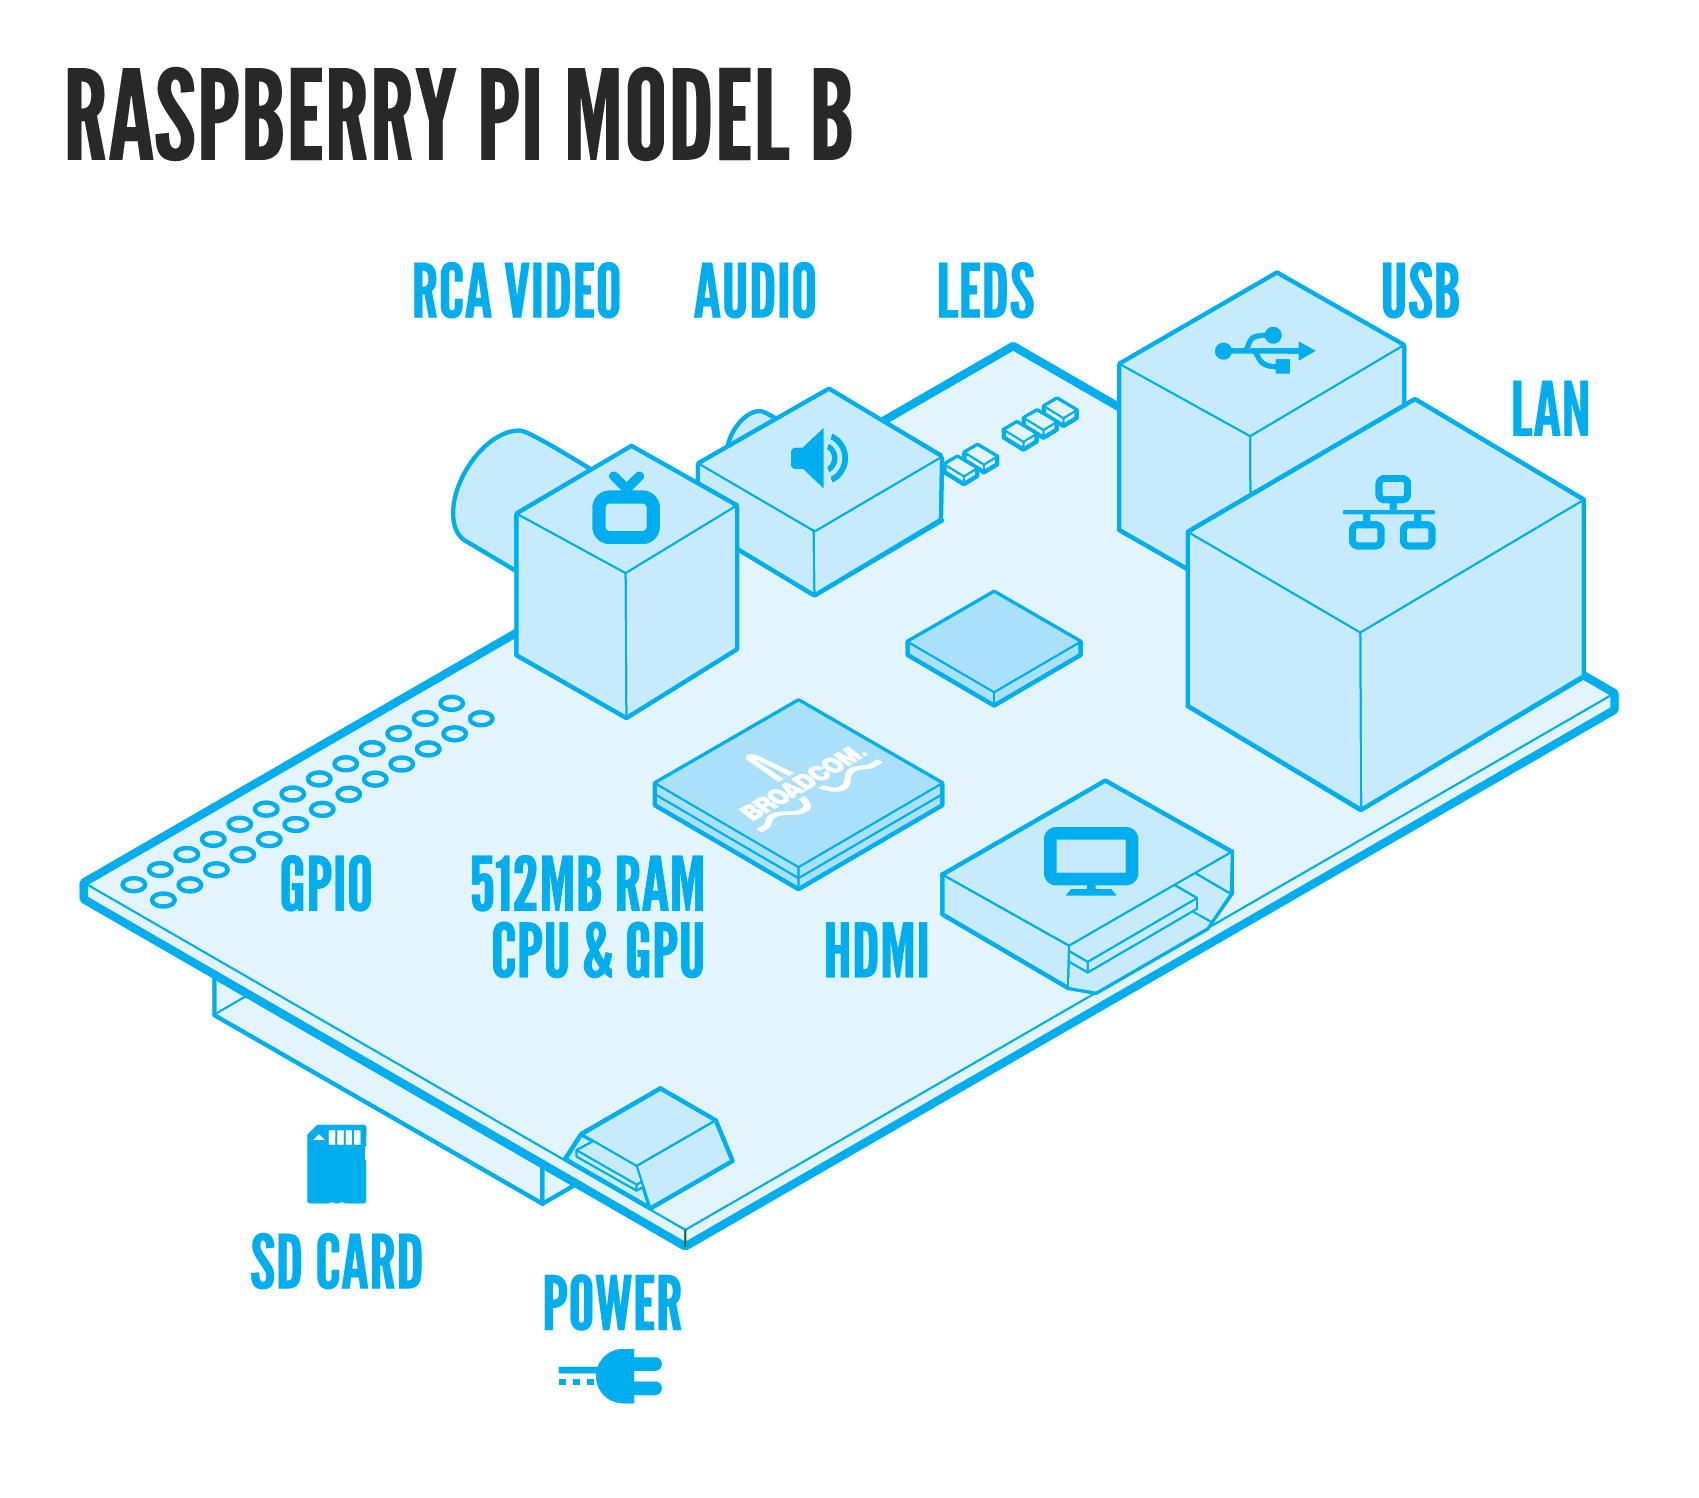
\includegraphics[width=0.80\textwidth]{figs/RaspiModelB.png}
  	\caption{Raspberry Pi used as Residential access point}
  	\label{fig:rpi}
\end{figure}

\subsection{\gls{rpi} Operation System}
\par The Raspberry Pi Foundation provides Debian and Arch Linux ARM distributions as \gls{rpi} operating system.Tools are available for Python as the main programming language on the \gls{rpi}, with support for BBC BASIC (via the RISC OS image or the "Brandy Basic" clone for Linux),C and Perl. In this project the recommended operating system, Raspbian wheezy\cite{raspbian} will be used as \gls{rpi} operating system. Raspbian is a free operating system based on Debian optimized for the Raspberry Pi hardware. An operating system is the set of basic programs and utilities that make Raspberry Pi run. However, Raspbian provides more than a pure OS: it comes with over 35,000 packages, pre-compiled software bundled in a nice format for easy installation on Raspberry Pi. For this prototype project, this kind of beginner operating system is best choice.

\section{Project Using Applications on Raspberry Pi}

\subsection{hostapd}
\par Most using package to provide Wifi hot-spot function on \gls{rpi} is hostapd\cite{hostapd} package. hostapd is an \gls{ieee} 802.11 \gls{ap} and \gls{ieee} 802.1X/\gls{wpa}/\gls{wpa2}/\gls{eap}/\gls{radius} Authenticator. The  advantages of using hostapd are that it is compatible well with the \gls{rpi} and it is easy to manually modified by script configuration file. The set up configuration file shows in Code Snippet\ref{code:hostapd_config}.

\begin{algorithm}[h]
  \caption{Code Snippet for hostapd configuration file}
  \label{code:hostapd_config}
  \begin{verbatim}
  
interface=wlan0
driver=nl80211
ctrl_interface=/var/run/hostapd
ctrl_interface_group=0
ssid=raspberry
hw_mode=g
channel=8
wpa=0
beacon_int=100
auth_algs=1
wmm_enabled=1
 \end{verbatim}
\end{algorithm}

\subsection{Dnsmasq}
\par For dynamically allocating \gls{ip} address for connected clients with \gls{rpi}, the protocol, \gls{dhcp} \cite{dhcp} is using in this project. \gls{dhcp} is a standardized networking protocol used on \gls{ip} addresses and other information that is needed for internet communication.\gls{dhcp} allows computers and other devices to receive an \gls{ip} address automatically from a central \gls{dhcp} server(\gls{rpi} in this project), reducing the need for a network administrator or a user from having to configure these settings manually. This working process is fit the requirement of prototype project because client users need have a \gls{ip} address to have the access to post internet access request to the central server then wait for the response of it. And the recommended networking protocol using in this case from the \gls{rpi} community is \gls{dhcp}.
\par In this project, on \gls{rpi} device, the application named dnsmasq \cite{dnsmasq} will be used to provide \gls{dns} forwarder and \gls{dhcp} server. For this prototype project, dnsmasq is a lightweight, easy to configure \gls{dns} forwarder and \gls{dhcp} server. It is designed to provide \gls{dns} and, optionally, \gls{dhcp}, to a small network, like the residential area wireless network in this report case.

\begin{algorithm}[h]
  \caption{Code Snippet for dnsmasq configuration}
  \label{code:dnsmasq_config}
  \begin{verbatim}
  
interface=wlan0

dhcp-range=unauth,10.0.0.65,10.0.0.94,2m
dhcp-option-force=unauth,1,255.255.255.224
dhcp-option-force=unauth,6,129.241.200.170,129.241.200.170

dhcp-range=auth,10.0.0.1,static,2m
dhcp-range=auth,10.0.0.2,10.0.0.63,2h
dhcp-option-force=auth,1,255.255.255.192
dhcp-option-force=auth,6,8.8.8.8,8.8.4.4

dhcp-hostsfile=/etc/dnsmasq.hosts
 \end{verbatim}
\end{algorithm}

\par The configuration file for dnsmasq is shown in Code Snippet \ref{code:dnsmasq_config}. For this project, we set unauthenticated \gls{ip} address in the range from 10.0.0.65 to 10.0.0.94, the the lease available time is two minutes. The other hand, the authenticated \gls{ip} address are in the range from 10.0.0.2 to 10.0.0.62. And for unauthenticated clients, the \gls{dns} server would be 129.241.200.170 which is central management server to redirect network traffic for each unauthenticated \gls{ip} address. For authenticated clients, the \gls{dns} server would be the Google Open \gls{dns} server to reduce the complexity of the \gls{rpi} residential access point. Moreover, we set the hosts file to '/etc/dnsmasq.hosts'. this file will store the static lease script. The example script in dnsmasq.hosts would be like Code Snippet \ref{code:dnsmasq_hosts}, it includes \gls{ip} address leased by the client user , \gls{macaddress} address from the client user device and the \gls{ip} lease available time. The dnsmasq hosts file would be modified when there is any changes from the central management server updating the client user authorization.

\begin{algorithm}[h]
  \caption{Code Snippet for dnsmasq hosts file}
  \label{code:dnsmasq_hosts}
  \begin{verbatim}
  
e4:ce:8f:03:7f:e0,10.0.0.6,2h
 \end{verbatim}
\end{algorithm}

\subsection{Iptables}
\par 
